\section{Experimental setup}
\label{Exp}
In this section, we first describe the datasets used for our experiments and the corresponding classification tasks. We then delineate the networks used for each of these datasets and the procedure to determine the values of hyperparameters. This is followed by a description of the evaluation metric of the speedup. All the algorithms were implemented in C++. The reported results were obtained on a Ubuntu 14.04.4 LTS system with 32 cores, 128 GB RAM and a clock speed of 2.6 GHz.  

\subsection{Dataset description}
\label{sub:data_desc}
We test the speedups achieved by the parallel implementation on two public datasets - MNIST and KDD Cup 1999. These datasets have been widely used by the machine learning community to compare different learning algorithms. Their description is as follows:

\begin{itemize}
\item \textbf{MNIST} - This is an image database of handwritten digits which is commonly used for training various image processing systems (Figure \ref{fig:mnist}). The task here is to classify the digit in the image. This dataset was derived from NIST's datasets and was formed by mixing the samples from NIST. This mixing was done because the training and testing datasets in the original NIST dataset were obtained from two different groups of people (Census Bureau employees and high school students). This dataset consists of 60,000 training images and 10,000 testing images, each of size 28$\times$ 28. In our experiments, we further divided the training set into training and validation in 5:1 ratio in order to determine suitable values for the hyperparameters.

\begin{figure}
  \centering
       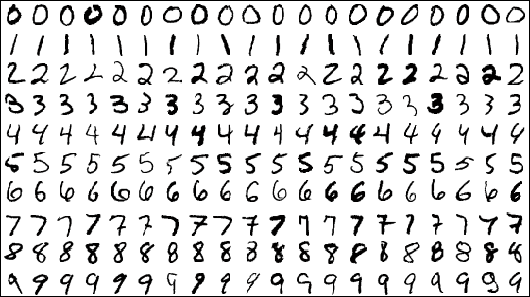
\includegraphics[scale=0.43]{mnist.png}
  \caption{MNIST dataset}
  \label{fig:mnist}
\end{figure}

\item \textbf{KDD Cup 1999} -  This is a dataset which first appeared in the KDD Cup held in 1999. The dataset has about 4 million data points each of which has 42 features. The features are of two types - categorical and integer. The task in the competition was to build a network intrusion detector which can be used to distinguish between good and bad network connections. 
\end{itemize}

\subsection{Network details}
\label{sub:net_det}
We now describe the details of the structure of neural networks used. For our experiments, we use two different configurations of neural network - 
\begin{itemize}
\item \textbf{Net-1h} - This network consists of 3 layers - input layer, one hidden layer and output layer. The input layer has 784 neurons for MNIST dataset and 42 neurons for KDD Cup 1999. The hidden layer is composed of 1024 neurons and the output layer has 10 neurons when used for MNIST dataset and 1 output for KDD Cup 1999.
\item \textbf{Net-2h} - This network is composed of 4 layers - input layer, two hidden layers and output layer. The input and output layer are same as Net-1h and each of the hidden layers has 1024 neurons.
\end{itemize}

\subsection{Hyperparameter selection}
\label{sub:hyper_sel}
Hyperparameter selection, also known as model selection, is an important problem in machine learning. It refers to choosing the optimal hyperparameters for a learning algorithm. It is crucial to select the values for hyperparameters which generalize well. This enables the algorithm to perform well on test data.

In the context of neural networks, hyperparameters refer to learning rate and regularization constant. Since our implementation is free of regularization, we only have one hyperparameter - learning rate. To choose an optimal learning rate, we used the technique of grid search. As mentioned above, we divide the training set into training and validation. We use different learning rates defined in a grid and test the accuracy on the validation data. The rate which gives the highest accuracy on validation is chosen and used to evaluate the performance of the algorithm on test data.

\subsection{Evaluation methodology}
\label{sub:eval}
As has been previously mentioned, this work aims to speed up the learning of neural network by parallelizing backpropagation and running it on GPU. To evaluate our approach and quantify the usefulness of parallelization, we use speed up as our primary measure. We calculate this with respect to the serial implementation on the same network configuration. Speed up may sometimes be misleading and does not capture the efficiency of serial implementation. To resolve this we use another measure - GFLOPS (Billion Floating Point Operations Per Second). This measure is independent of serial implementation and can be used to supplement the speedup metric.

\subsection{Experiments}
\label{sub:exp}
In this paper, we implement the gradient descent algorithm for training neural network. The implementation is 3-fold - serial, parallelization with Pthreads and parallelization with CUDA. The implementation follows from section \ref{BackProp} and section \ref{GPUBackProp}. Please refer to these sections for a detailed explanation of the methods.


